\documentclass{beamer}
%\documentclass[handout]{beamer}

\usetheme{Copenhagen}
%\usetheme{Darmstadt}
%\usecolortheme{crane}
%\usecolortheme{dove}
\usecolortheme{dolphin}

%\usepackage{default}
\usepackage{graphicx}
\usepackage{algorithmic,algorithm}
\usepackage{amssymb}
\usepackage{amsmath}
\usepackage{amsthm}
\usepackage{graphicx}

\def\versio{Versi\'o 0.9.0\\}%

\setbeamercovered{transparent}

 %%% Abreviaturas
\def\lgem{l\ensuremath{\cdot}l}
\def\ce{corba e\lgem{}\'{\i}ptica}%
\def\ces{corbes e\lgem{}\'{\i}ptiques}%
\def\CE{Corba E\lgem{}\'{\i}ptica}%
\def\CEs{Corbes E\lgem{}\'{\i}ptiques}%
\def\cf{cos finit}%
\def\cfs{cossos finits}%
\def\Cfs{Cossos finits}%
\def\Cf{Cos finit}%
\def\sgc{subgrup c\'{\i}clic}%
\def\Sgc{Subgrup c\'{\i}clic}%
\def\ecdlp{logaritme discret e\lgem{}\'{\i}ptic}%


%%% Definiciones matem\'aticas especiales

\newcommand{\Z}{\ensuremath{\mathbb{Z}}}%			Enteros
\newcommand{\Q}{\ensuremath{\mathbb{Q}}}%			Racionales
\newcommand{\R}{\ensuremath{\mathbb{R}}}%			Reales
\newcommand{\C}{\ensuremath{\mathbb{C}}}%			Complejos
\newcommand{\A}{\ensuremath{\mathbb{A}_{2}}}%			Plano Af\'{\i}n
\newcommand{\Proy}{\ensuremath{\mathbb{P}_{2}}}%		Plano Proyectivo
\newcommand{\K}{\ensuremath{\mathbb{K}}}%			Cuerpo en general
\newcommand{\F}{\ensuremath{\mathbb{F}}}%			Cuerpo finito en general
\newcommand{\Fp}{\ensuremath{\mathbb{F}_p}}%			Cuerpo finito de orden p (primo)
\newcommand{\EFp}{\ensuremath{E(\mathbb{F}_p)}}%		Curva el\'\{i}ptica sobre un cuerpo finito de orden p (primo)
\newcommand{\EFpbis}{\ensuremath{E/\mathbb{F}_p}}
\newcommand{\Fm}{\ensuremath{\mathbb{F}_{2^m}}}%                Cuerpo finito de caractar\'{\i}stica 2, grado m
\newcommand{\Fq}{\ensuremath{\mathbb{F}_q}}%			Idem id. q (q=p^m, p primo y m entero pos.)
\newcommand{\Zn}[1]{\ensuremath{\mathbb{Z}/#1\mathbb{Z}}}%	Anillo de los enteros mod n
\newcommand{\PaI}{\ensuremath{\mathcal{O}}}%                    Punto en el Infinito
\newcommand{\PaIe}{\ensuremath{\mathcal{O}_{E}}}%               Punto en el Infinito de la curva

%%%% ``Castellanizaci\'on'' de 'algorithmic.sty'

\renewcommand{\algorithmicrequire}{\textbf{Prerequisit:}}%
\renewcommand{\algorithmicensure}{\textbf{Postrequisit:}}%
\renewcommand{\algorithmiccomment}[1]{/* #1 */}%	
\renewcommand{\algorithmicend}{\textbf{fi}}%
\renewcommand{\algorithmicif}{\textbf{si}}%
\renewcommand{\algorithmicthen}{\textbf{llavors}}%
\renewcommand{\algorithmicelse}{\textbf{si no}}%
\renewcommand{\algorithmicfor}{\textbf{per}}%
\renewcommand{\algorithmicforall}{\textbf{per a tot}}%
\renewcommand{\algorithmicdo}{\textbf{fer}}%
\renewcommand{\algorithmicwhile}{\textbf{mentre}}%
\renewcommand{\algorithmicloop}{\textbf{bucle}}%
\renewcommand{\algorithmicrepeat}{\textbf{repetir}}%
\renewcommand{\algorithmicuntil}{\textbf{fins}}%

\floatname{algorithm}{Algorisme}%

% %%% Teoremas y dem\'as
% \theoremstyle{plain}        			% Cargar el paquete theorem.sty o amsthm.sty
 
% \theoremstyle{definition}   			% Cargar el paquete amsthm.sty
 
 \newtheoremstyle{saltolinea}% name   		% Sacado del 'thmtest.tex'
   {9pt}%               Space above, empty = `usual value'
   {9pt}%               Space below
   {}%                  Body font
   {}%                  Indent amount (empty = no indent, \parindent = para indent)
 %  {\bfseries}%         Thm head font
   {\scshape}%          Thm head font
   {}%                  Punctuation after thm head
   {\newline}%          Space after thm head: \newline = linebreak
   {}%                  Thm head spec
 
 \theoremstyle{saltolinea}   			% Cargar el paquete amsthm.sty
 \newtheorem{algo}{Algorisme}

\title{Criptografia lliure amb \ces{}}
%\author[Sergi Blanch i Torn\'e]{Sergi Blanch i Torn\'e \\ sblanch@alumnes.udl.cat}
\date{Setembre, 2008}

\begin{document}

%%%%%%%%%%%%
%\frame{\titlepage}
\begin{frame}
  \begin{block}{}
    \begin{huge}\begin{center}Criptografia lliure\\ amb \ces{}\end{center}\end{huge}
  \end{block}
  \begin{columns}[t]
    \column{.5\textwidth}
      \begin{block}{Estudiant}
         Sergi \textsc{Blanch i Torn\'e}
      \end{block}
    \column{.5\textwidth}
      \begin{block}{\begin{flushright}Director\end{flushright}}
         \begin{flushright}Ramiro \textsc{Moreno Chiral}\end{flushright}
      \end{block}
  \end{columns}
  \begin{center}
    Setembre, 2008
  \end{center}
\end{frame}
%%%%%%%%%%%%

%%%%%%%%%%%%
\begin{frame}
  \frametitle{Outline}
  \transdissolve
  \tableofcontents[hideallsubsections]
\end{frame}
%%%%%%%%%%%%

%%%%%%%%%%%%%%%%%%%%%%%%%%%%%%%%%%%%
%\section{Aritm\`etica de \ce}

%%%%%%%%%%%%%%%%%%%%%%%%%%%%%%%%%%%%
%\subsection{\Cfs{} de caracter\'{\i}stica prima}

%%%%%%%%%%%%%%%%%%%%%%%%%%%%%%%%%%%%
%\subsection{Plans afins i projectius}

%%%%%%%%%%%%%%%%%%%%%%%%%%%%%%%%%%%%
%\subsection{Definint \ces}

%%%%%%%%%%%%%%%%%%%%%%%%%%%%%%%%%%%%
%\subsubsection{\ecdlp}

%%%%%%%%%%%%%%%%%%%%%%%%%%%%%%%%%%%%
\section{Criptografia amb \ces}

%%%%%%%%%%%%
\begin{frame}
  \frametitle{Setup d'un criptosistema}
  %\transdissolve
  \begin{columns}[H]
    \column{.5\textwidth}
      \begin{block}{Requisits}
        \begin{itemize}
          \item<2-> \EFp
          \item<2-> $y^2=x^3+ax+b$
          \item<4-> $\left\langle G\right\rangle = \left\{ G,[2]G,[3]G,\ldots\right\}$
          \item<6-> $n = ord(G)$ ($[n]G=\mathcal{O}_{E}$)
          \item<8-> $|\EFp| = n \cdot h$
        \end{itemize}
      \end{block}
    \column{.5\textwidth}
      \begin{block}{Tupla}
        \begin{itemize}
          \item<3-> $p$
          \item<3-> $a$, $b$
          \item<5-> $G$
          \item<7-> $n$
          \item<9-> $h$
        \end{itemize}
      \end{block}
  \end{columns}
\end{frame}
%%%%%%%%%%%%

%%%%%%%%%%%%%%%%%%%%%%%%%%%%%%%%%%%%
\subsection{Normatives}

%%%%%%%%%%%%
\begin{frame}
  \frametitle{Normatives (I)}
  %\transdissolve
  \begin{itemize}
    \item<2-> ``P1363''
    \begin{itemize}
      \item<3-> del IEEE: \emph{Institute of Electrical and Electronics Engineers}
      \item<4-> Draft 1994
      \item<5-> Definitiva 2000
      \item<6-> Ampliada amb la P1363a, 1363.1, 1363.2, 1363.3
      \item<7-> Especificacions i implementacions d'algorismes en llenguatge formal
      \begin{itemize}
        \item<8-> Plans afin (\A) i projectiu (\Proy)
        \item<9-> \CEs{} sobre \\
          \cfs{} primers \Fp \\
          \cfs{} de caracter\'{\i}stica 2 \Fm
      \end{itemize}
      \item<10-> Precauci\'o amb les patents
    \end{itemize}
  \end{itemize}
\end{frame}
%%%%%%%%%%%%

%%%%%%%%%%%%
\begin{frame}
  \frametitle{Normatives (II)}
  %\transdissolve
  \begin{itemize}
    \item<1-> ``FIPS 186''
    \begin{itemize}
      \item<2-> del NIST: \emph{National Institute of Standards and Technology}
      \item<3-> Evoluciona: actualment 186-3 (2006)
      \item<4-> Especifica el setup recomanat per us federal
      \begin{itemize}
        \item<5-> Corbes de Koblitz
        \item<6-> Corbes sobre \Fm
        \item<7-> Corbes sobre \Fp
      \end{itemize}
    \end{itemize}
  \end{itemize}
\end{frame}
%%%%%%%%%%%%

%%%%%%%%%%%%
\begin{frame}
  \frametitle{Normatives (i III)}
  %\transdissolve
  \begin{itemize}
    \item<1-> ``ECC in OpenPGP''
    \begin{itemize}
      \item<2-> del IEFT: \emph{Internet Engineering Task Force}
      \item<3-> Extensi\'o del rfc4880 \emph{OpenPGP Message Format}
      \item<4-> Est\`andard d'interoperabilitat entre aplicacions
      \item<5-> Utilitza corbes del NIST
      \begin{itemize}
        \item<6-> \emph{P-256}: $\sim 3072$ RSA. Considerat per dades \emph{``Secret''}
        \item<7-> \emph{P-384}: $\sim 7680$ RSA. Considerat per dades \emph{``Top Secret''}
        \item<8-> \emph{P-521}: $\sim 15360$ RSA
      \end{itemize}
      \item<9-> Algorisme de xifrat pr\`oxim al ECDH+AES256
      \item<10-> Ser\`a oficial al Novembre (o expira al Gener)
    \end{itemize}
  \end{itemize}
\end{frame}
%%%%%%%%%%%%

%%%%%%%%%%%%%%%%%%%%%%%%%%%%%%%%%%%%
\subsection{Firma digital ECDSA}

%%%%%%%%%%%%
\begin{frame}
  %\transdissolve
  \begin{algo}[Signatura ECDSA]\label{alg:ECDSA}
    \parbox[b]{\linewidth}{%
      {\bf INPUT}: Clau secreta $skey_{M}$ i hash del missatge $\#hash$.\\
      {\bf OUTPUT}: Parell $\left(r,s\right)$/{*}tal que $0<r,s<skey_{A}.n${*}/.
      \hrule
    }%
    \vspace{-7mm}
    \begin{algorithmic}[1]
      \STATE Generar aleatoriament una clau de sessi\'o $k\in_{R}\left[1,\left(skey_{M}.p\right)-2\right]$;
      \STATE \alert<2>{$I\leftarrow \left[k\right]\left(skey_{M}.G\right)$;}
      \STATE $i\leftarrow I_{x}$;
      \STATE $r\leftarrow i\left(mod\: skey_{M}.n\right)$;
      \STATE si $r=0$ llavors goto 1;
      \STATE $s\leftarrow k^{-1}\cdot\left(\# hash+\left(skey_{M}.d\right)\cdot r\right)\left(mod\: skey_{M}.n\right)$;
      \STATE Si $s=0$ llavors goto 1;
      \STATE Return $(r,s)$;
    \end{algorithmic}
  \end{algo}%
\end{frame}
%%%%%%%%%%%%

%%%%%%%%%%%%
\begin{frame}
  %\transdissolve
  \begin{algo}[Verificaci\'o ECDSA]\label{alg:ECDSA_verif}
    \parbox[b]{\linewidth}{%
      {\bf INPUT}: Clau p\'ublica $pkey_{M}$, hash $\#hash$ i el parell $\left(r,s\right)$.\\
      {\bf OUTPUT}: Boole\`a d'acceptaci\'o o rebuig.
      \hrule
    }%
    \vspace{-7mm}
    \begin{algorithmic}[1]
      \STATE Verificar $\left(r,s\right)\in\left[1,\left(pkey_{M}.n\right)-1\right]$;
      \STATE $h\leftarrow s^{-1}\left(mod\: pkey_{M}.n\right)$;
      \STATE $h_{1}\leftarrow\left(\# hash\right)\cdot h\left(mod\: pkey_{M}.n\right)$;
      \STATE $h_{2}\leftarrow r\cdot h\left(mod\: pkey_{M}.n\right)$;
      \STATE \alert<2>{$Q\leftarrow \left[h_{1}\right]\left(pkey_{M}.G\right)+\left[h_{2}\right]\left(pkey_{M}.G\right)$;}
      \STATE Si $Q=\mathcal{O}_{E}$ llavors refuse;
      \STATE $i\leftarrow Q_{x}\left(mod\: pkey_{M}.n\right)$;
      \STATE Si $i=r$ llavors accept; sin\'o refuse;
    \end{algorithmic}
  \end{algo}%
\end{frame}
%%%%%%%%%%%%

%%%%%%%%%%%%%%%%%%%%%%%%%%%%%%%%%%%%
\subsection{Xifrat}

%%%%%%%%%%%%%%%%%%%%%%%%%%%%%%%%%%%%
\subsubsection{ECElGamal}

%%%%%%%%%%%%
\begin{frame}
  %\transdissolve
  \begin{algo}[Xifrat ElGamal el$\cdot$l\`{\i}ptic]\label{alg:ECElGamal}
    \parbox[b]{\linewidth}{%
      {\bf INPUT}: Clau p\'ublica $pkey_{M}$ i l'enter a xifrar $z$.\\
      {\bf OUTPUT}: Xifrat formar per un parell de punts, $(R,C)$.
      \hrule
    }%
    \vspace{-7mm}
    \begin{algorithmic}[1]
      \STATE Generar aleatoriament una clau de sesi\'o $k\in_{R}\left[1,\left(pkey_{M}.n\right)-1\right]$;
      \STATE \alert<2>{$R \leftarrow \left[k\right] pkey_{M}.G$;}
      \STATE \alert<3>{$Q \leftarrow \left[k\right] pkey_{M}.P$;} \alert<4>{\COMMENT{$P=\left[d\right] G$; $Q=\left[k\right] (\left[d\right] G)$}}
      \STATE \alert<5>{Convertir el missatge a punt de la \ce{} $z\rightarrow Z$;}
      \STATE $C \leftarrow Z+Q$;\label{alg:ECElGamal:suma}
      \STATE Return $(R,C)$;
    \end{algorithmic}
  \end{algo}
\end{frame}
%%%%%%%%%%%%

%%%%%%%%%%%%%%%%%%%%%%%%%%%%%%%%%%%%
\subsubsection{ECDH+AES256}

%%%%%%%%%%%%
\begin{frame}
  %\transdissolve
  \begin{algo}[Xifrat ECDH+AES256]\label{alg:ecdhAES256}
    \parbox[b]{\linewidth}{%
      {\bf INPUT}: Clau p\'ublica $pkey_{M}$ i text en clar num\'eric $z$.\\
      {\bf OUTPUT}: Parell punt resultant $R$ i xifra $c$.
      \hrule
    }%
    \vspace{-7mm}
    \begin{algorithmic}[1]
      \STATE Generar aleatoriament una clau de sesi\'o $k\in_{R}\left[1,\left(pkey_{M}.n\right)-1\right]$;
      \STATE $R \leftarrow \left[k\right] pkey_{M}.G$;
      \STATE $Q \leftarrow \left[k\right] pkey_{M}.P$; %\COMMENT{$P=\left[d\right] G$; $Q=\left[k\right] (\left[d\right] G)$}
      \STATE \alert<2>{$c \leftarrow \textrm{aes256}(z,\textrm{sha256}(Q_x))$;}
      \STATE Return $(R,c)$;
    \end{algorithmic}
  \end{algo}
\end{frame}
%%%%%%%%%%%%

%%%%%%%%%%%%%%%%%%%%%%%%%%%%%%%%%%%%
\subsubsection{EccOpenPGP}

%%%%%%%%%%%%
\begin{frame}
  %\transdissolve
  \begin{algo}[Xifrat ECC\_OpenPGP]\label{alg:eccOpenPGP}
    \parbox[b]{\linewidth}{%
      {\bf INPUT:}: Clau p\'ublica $pkey_{M}$ i text en clar num\'eric $z$.\\
      {\bf OUTPUT}: Parell punt resultant $R$ i xifra $c$.
      \hrule
    }%
    \vspace{-7mm}
    \begin{algorithmic}[1]
      \STATE Generar aleatoriament una clau de sessi\'o $k\in_{R}\left[1,\left(pkey_{M}.n\right)-1\right]$;
      \STATE $R \leftarrow \left[k\right] pkey_{M}.G$
      \STATE $S \leftarrow \left[k\right] pkey_{M}.P$; \COMMENT{$S=\left[k\right] (\left[d\right] G)=\left[d\right] (\left[k\right]\cdot G)=\left[d\right]\cdot K$}
      \STATE $\textrm{Param}  \leftarrow \textrm{curveID} || \textrm{pubkeyID} || 01 || \textrm{KDF\_hashID} || $\\$ \textrm{aesID} || \textrm{``AnonymousSender''} || \textrm{recipient\_fingerprint}$;
      \STATE \alert<2>{$Z \leftarrow KDF\left(S,len\left(aesID\right),Param\right)$;\label{alg:eccOpenPGP:kdf}}
      \STATE \alert<3>{$c \leftarrow \textrm{AESkeyWrap}\left(Z,\textrm{m}\right)$;}
      \STATE Return $(R,c)$;
    \end{algorithmic}
  \end{algo}
\end{frame}
%%%%%%%%%%%%

%%%%%%%%%%%%
\begin{frame}
  %\transdissolve
  \begin{algo}[Key Derivation Function]\label{alg:KDF}
    \parbox[b]{\linewidth}{%
      {\bf INPUT:}: Punt $S$, longitud de l'output $obits$ i cadena $Param$.\\
      {\bf OUTPUT}: cadena de bits.
      \hrule
    }%
    \vspace{-7mm}
    \begin{algorithmic}[1]
      \STATE $\textrm{cntr}  \leftarrow  1$;
      \STATE $\textrm{threshld}  \leftarrow \left(obits+hbits-1)/hbits\right)$;
      \REPEAT
      \STATE $\textrm{C32} \leftarrow \left(\textrm{unit32}\right)\textrm{big\_endian}\left(\textrm{cntr}\right)$;
      \STATE $\textrm{HB} \leftarrow \textrm{hash}\left(S_{x} || C32 || Param\right)$;
      \STATE $\textrm{MB} \leftarrow \textrm{MB} || \textrm{HB}$;
      \UNTIL {$\textrm{cntr} \leq \textrm{threshold}$};
      \STATE return leftmost obits of MB
    \end{algorithmic}
  \end{algo}
\end{frame}
%%%%%%%%%%%%

%%%%%%%%%%%%
\begin{frame}
  %\transdissolve
  \begin{algo}[Desxifrat ECC\_OpenPGP]\label{alg:deseccOpenPGP}
    \parbox[b]{\linewidth}{%
      {\bf INPUT:}: Clau privada $skey_{M}$ i parell d'elements xifra $\left(R,c\right)$.\\
      {\bf OUTPUT}: Text pla $z$.
      \hrule
    }%
    \vspace{-7mm}
    \begin{algorithmic}[1]
      \STATE $S \leftarrow \left[skey_{M}.d\right] R$;
      \STATE $\textrm{Param}  \leftarrow \textrm{curveID} || \textrm{pubkeyID} || 01 || \textrm{KDF\_hashID} || $\\$ \textrm{aesID} || \textrm{``AnonymousSender''} || \textrm{recipient\_fingerprint}$;
      \STATE $Z \leftarrow KDF\left(S,len\left(aesID\right),Param\right)$;\label{alg:deseccOpenPGP:kdf}
      \STATE $m \leftarrow \textrm{AESkeyWrap}^{-1}\left(Z,\textrm{c}\right)$;
      \STATE Return $m$;
    \end{algorithmic}
  \end{algo}
\end{frame}
%%%%%%%%%%%%

%%%%%%%%%%%%%%%%%%%%%%%%%%%%%%%%%%%%
\section{Criptoan\`alisis el$\cdot$l\'{\i}ptic}

%%%%%%%%%%%%
\begin{frame}
  %\transdissolve
  \frametitle{Criptoan\`alisis el$\cdot$l\'{\i}ptic (I)}
  \begin{itemize}
    \item<1-> Atacs directes
    \begin{itemize}
      \item<2-> For\c{c}a bruta
      \begin{itemize}
        \item<2-> $O\left(n\right)$
      \end{itemize}
      \item<3-> Baby step / Giant Step
      \begin{itemize}
        \item<3-> $O\left(\sqrt[4]{n}\right)$ En mem\`oria i comput
      \end{itemize}
      \item<4-> Rho ($\rho$) de Pollard
      \begin{itemize}
        \item<4-> $O\left(\sqrt[4]{n}\right)$ En comput, $O\left(1\right)$ en mem\`oria
      \end{itemize}
      \item<5-> Index Calculus i Xedni Calculus
      \begin{itemize}
        \item<5-> Menor que $O\left(n^\alpha\right)$ sense arribar a $O\left(log^{\alpha}n\right)$
        \item<6-> No es aplicable a \ces
      \end{itemize}
      \item<7-> Pohlig-Hellman
      \begin{itemize}
        \item<8-> Cas que l'ordre del grup factoritzi: \\
         $n = \mathrm{ord}(G)= \prod_{i=1}^{k} {p_{i}}^{e_{i}},$
        \item<8-> $O\left(\sqrt{p_{i}}\right)$ on $p_{i}$ \'es el m\'es gran dels factors
      \end{itemize}
    \end{itemize}
  \end{itemize}
\end{frame}
%%%%%%%%%%%%

%%%%%%%%%%%%
\begin{frame}
  %\transdissolve
  \frametitle{Criptoan\`alisis el$\cdot$l\'{\i}ptic (i II)}
  \begin{itemize}
    \item<1-> Atacs laterals
    \begin{itemize}
      \item<2-> Actius
      \begin{itemize}
        \item<3-> Temps de resposta
        \item<3-> Missatge escollit
      \end{itemize}
      \item<4-> Pasius
      \begin{itemize}
        \item<5-> Consum el\`ectic d'operacions iteratives
        \item<5-> An\`alisis lineal
        \item<5-> An\`alisis diferencial
      \end{itemize}
    \end{itemize}
  \end{itemize}
\end{frame}
%%%%%%%%%%%%

%%%%%%%%%%%%%%%%%%%%%%%%%%%%%%%%%%%%
\subsection{Atacs directes}

%%%%%%%%%%%%%%%%%%%%%%%%%%%%%%%%%%%%
\subsection{Atacs laterals}

%%%%%%%%%%%%
\begin{frame}
  %\transdissolve
  \frametitle{Atacs laterals}
  \begin{enumerate}
    \item<2-> \textbf{NO} ataquen la matem\`atica
    \item<3-> Ataquen l'implementaci\'o
    \item<4-> Afecten:
    \begin{itemize}
      \item<5-> Sistemes de mem\`oria compartida
      \begin{itemize}
        \item<6-> multiples fils d'execuci\'o
        \item<6-> mem\`oria cau no protegida
      \end{itemize}
      \item<7-> sistemes monousuari
      \begin{itemize}
        \item<8-> Targetes intel$\cdot$ligent
        \item<8-> Sistemes empotrats
      \end{itemize}
    \end{itemize}
  \end{enumerate}
\end{frame}
%%%%%%%%%%%%

%%%%%%%%%%%%%%%%%%%%%%%%%%%%%%%%%%%%
\subsection{Atacs actius}

%%%%%%%%%%%%
\begin{frame}
  %\transdissolve
  \frametitle{Atacs actius}
  Extreute informaci\'o privada en base a comportaments de caixa negra:
  \begin{itemize}
    \item<2-> Temps de resposta
    \item<3-> Missatge escollit
  \end{itemize}
\end{frame}
%%%%%%%%%%%%

%%%%%%%%%%%%%%%%%%%%%%%%%%%%%%%%%%%%
\subsection{Atacs passius}

%%%%%%%%%%%%
\begin{frame}
  %\transdissolve
  \frametitle{Atacs passius}
  \begin{itemize}
    \item<2-> Extreure informaci\'o privada de l'entorn
    \begin{itemize}
      \item<3-> Consum el\`ectric distingible segons l'operaci\'o que s'efectua
      \item<4-> Busqueda de patrons
      \item<5-> Superposici\'o de mostres
    \end{itemize}
    \item<6-> Primeres contramesures
    \begin{itemize}
      \item<7-> Canvi variable en la freq\"u\`encia de rellotge
      \item<8-> Introdueix el criptoan\`alisis difer\`encial
    \end{itemize}
  \end{itemize}
\end{frame}
%%%%%%%%%%%%

%%%%%%%%%%%%%%%%%%%%%%%%%%%%%%%%%%%%
\subsection{Proteccions i contramesures}

%%%%%%%%%%%%
\begin{frame}
  %\transdissolve
  \frametitle{Proteccions i contramesures al m\`odul eccGnuPG}
  \begin{itemize}
    \item<2-> Varietat d'entorn d'execuci\'o
    \begin{itemize}
      \item<3-> Sistemes multiusuari
      \item<3-> Sistemes monousuari
    \end{itemize}
    \item<4-> Proteccions implementades:
    \begin{itemize}
      \item<5-> Sistema de xifrat ECDH+AES256
      \item<5-> Xifrat de blocs CBC
      \item<5-> Us de les coordenades projectives
      \item<5-> Isomorfismes de generadors per al \sgc
    \end{itemize}
  \end{itemize}
\end{frame}
%%%%%%%%%%%%

%%%%%%%%%%%%%%%%%%%%%%%%%%%%%%%%%%%%
\section{Estrelles d'isog\`enies}

% %%%%%%%%%%%%%%%%%%%%%%%%%%%%%%%%%%%%
% \subsection{Isomorfismes i isog\`enies}
% 
% %%%%%%%%%%%%%%%%%%%%%%%%%%%%%%%%%%%%
% \subsection{Volcans, serraladades i estrelles de \ce}

%%%%%%%%%%%%%%%%%%%%%%%%%%%%%%%%%%%%
\subsection{Possibilitats de l'\'us d'estrelles de \ces}

%%%%%%%%%%%%
\begin{frame}
  %\transdissolve
  \frametitle{Perqu\`e volem usar estrelles?}
  \begin{columns}
    \column{.4\textwidth}
      \begin{center}
        \begin{block}{Estructura de clau}<2->
           \begin{itemize}
             \item \alert<5>{$p$} \onslide<5>{$\rightarrow$ \EFp}
             \item \alert<6>{$a$,$b$} \onslide<6>{$\rightarrow$ Isog\`enia}
             \item \alert<4>{$\left< G \right>$} \onslide<4>{$\rightarrow$ Isomorfisme}
             \item $n$,$h$
%             \hline
             \item \alert<3>{$d$}
             \item \alert<3>{$P$} \onslide<3>{$= \left[d\right]G$}
           \end{itemize}
        \end{block}
      \end{center}
  \end{columns}
\end{frame}
%%%%%%%%%%%%

%%%%%%%%%%%%
\begin{frame}
  %\transdissolve
  \frametitle{Com les volem usar?}
  \begin{columns}[H]
    \column{.5\textwidth}
      \begin{center}
        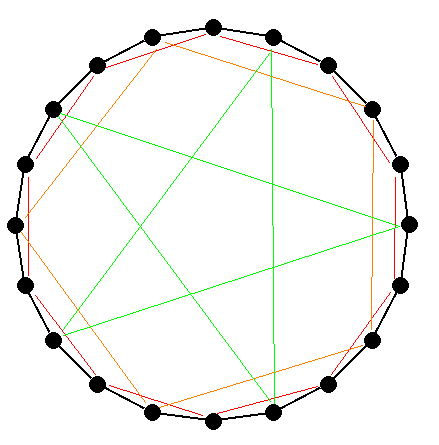
\includegraphics[width=.8\textwidth]{imatges/estrella2.png}
      \end{center}
    \column{.5\textwidth}
      \begin{algo}[Procediment de Setting d'una \ce{}]\label{alg:isogenia}
        \parbox[b]{\linewidth}{%
          \smallskip
          {\bf INPUT:}: $p$,$a_0$,$b_0$\\
          {\bf OUTPUT}: $a'$,$b'$
          \hrule
        }%
        \vspace{-7mm}
        \begin{algorithmic}[1]
          \STATE $k \in_R \mathbb{Z}_{>0}$
          \STATE $L=\left\{l_{0}^{e_{0}},l_{1}^{e_{1}},\dots,l_{k}^{e_{k}}\right\}$
          \STATE \alert<2>{$E' \leftarrow L\left(E_{0}\right)$;}
          \STATE Retornar $E'$;
        \end{algorithmic}
      \end{algo}
  \end{columns}
  \begin{block}{[PkIso]}<3>
    $\mathbb{F}_{2038074743} \rightarrow 30$ bits
  \end{block}
\end{frame}
%%%%%%%%%%%%

%%%%%%%%%%%%
\begin{frame}
  %\transdissolve
  \begin{columns}[H]
    \column{.9\textwidth}
      \begin{center}
        \begin{block}{Requeriments previs a l'implementaci\'o}
          \begin{itemize}
            \item<2-> Estudi del cost del c\`alcul
            \begin{itemize}
              \item<3-> Sobre les corbes del NIST: \\ \onslide<4->{P-192, P-224, P-256, P384, P-521}
              \item<5-> Sobre les corbes de brainpool:\\ \onslide<6->{P160r1,P192r1,P224r1,P256r1,P320r1,P384r1,P512r1}
              \item<7-> Proposta de noves corbes bones per isog\`enies
              \item<8-> Precauci\'o sobre les patents
            \end{itemize}
            \item<9-> Precodi
            \begin{itemize}
              \item<10-> LiDIA
              \item<11-> SciPy
              \item<12-> Sage
            \end{itemize}
          \end{itemize}
        \end{block}
      \end{center}
  \end{columns}
\end{frame}
%%%%%%%%%%%%

%%%%%%%%%%%%%%%%%%%%%%%%%%%%%%%%%%%%
\section{Gnu Privacy Guard}

%%%%%%%%%%%%%%%%%%%%%%%%%%%%%%%%%%%%
\subsection{Assignment - GNU GPG}

%%%%%%%%%%%%
\begin{frame}
  %\transdissolve
  \frametitle{Assignment - GNU GPG}
  \begin{itemize}
    \item<2-> Projecte llicenciat sota \emph{GPL}
    \begin{itemize}
      \item<3-> Co\lgem{}aboraci\'o \textbf{a} la comunitat
      \item<4-> Co\lgem{}aboraci\'o \textbf{de} la comunitat
    \end{itemize}
      \item<5-> Feature request
  \end{itemize}
\end{frame}
%%%%%%%%%%%%

%%%%%%%%%%%%%%%%%%%%%%%%%%%%%%%%%%%%
\subsection{Dos branques, dos codis}

%%%%%%%%%%%%
\begin{frame}
  %\transdissolve
  \frametitle{Gnu Privacy Guard}
  \begin{itemize}
    \item<2-> GnuPG 1.4
    \item<3-> GnuPG 2.0
    \begin{itemize}
      \item<4-> libassuan
      \item<5-> libksba
      \item<6-> libgcrypt
      \item<7-> libgpg-error
    \end{itemize}
  \end{itemize}
\end{frame}
%%%%%%%%%%%%

%%%%%%%%%%%%
\begin{frame}
  %\transdissolve
  \frametitle{Dos branques, dos codis}
  \begin{itemize}
    \item<2-> \emph{eccGnuPG} versi\'o 0.2.0 per al \emph{GnuPG} 1.4.9
    \item<3-> \emph{libgcrypt} 1.4.3
  \end{itemize}
  \begin{itemize}
    \item<4-> Estructures de dades diferents
    \item<5-> Primitives diferents
    \item<6-> Depend\`encies a llibreries
  \end{itemize}
\end{frame}
%%%%%%%%%%%%

%%%%%%%%%%%%%%%%%%%%%%%%%%%%%%%%%%%%
\section{Conclusions i treball futur}

%%%%%%%%%%%%
\begin{frame}
  %\transdissolve
  \frametitle{Conclusions i treball futur}
    \begin{itemize}
      \item<2-> Feina feta
      \begin{itemize}
        \item<3-> Desembolupament d'un xifrat robust
        \item<4-> Protecci\'o als atacs laterals
        \item<5-> Introducci\'o del projecte en el desembolupament oficial
        \item<6-> Optimitzaci\'o de les operacions
      \end{itemize}
    \end{itemize}
    \begin{itemize}
      \item<7-> Feina oberta
      \begin{itemize}
        \item<8-> Implementaci\'o de l'est\`andard ``\emph{Ecc in OpenPGP}''
        \item<9-> Optimitzaci\'o de les isog\`enies de \ce{}
        \item<10-> Proposici\'o d'est\`andard per a les isog\`enies
      \end{itemize}
    \end{itemize}
\end{frame}
%%%%%%%%%%%%

\end{document}
